%----------------------------------------------------------------------------
\chapter{\bevezetes}
\label{ch:bevezetes}
%----------------------------------------------------------------------------

A kosárlabda az egyik legnépszerűbb sportág világszerte, amelyben a büntetődobás kritikus szerepet játszik a mérkőzések végkimenetelében. Mivel a büntetődobás egy zavartalan, rögzített távolságból végrehajtott statikus mozdulatsor, a sikeres végrehajtást szinte kizárólag a játékos technikája és biomechanikai mozgásmintája határozza meg. A magas szintű teljesítmény eléréséhez elengedhetetlen a mozgás optimalizálása, a dobás konzisztenciájának javítása és a hibák azonosítása.

\section{Irodalomkutatás}
A kosárlabda büntetődobás kinematikai és biomechanikai sajátosságait a sporttudomány évtizedek óta vizsgálja \cite{Hudson1985}. A sikeres dobás egyik legfontosabb tényezője az optimális elengedési paraméterek (release conditions) megléte: az elengedési szög, az elengedési magasság és az elengedési sebesség \cite{Tran2008}. Az irodalom egyetért abban, hogy a jobb találati arány eléréséhez a magasabb elengedési pont és a megfelelő belépési szög biztosítása szükséges \cite{Miller1996, AgudoOrtega2014}. 

Továbbá a mozgás koordinációja és variabilitása is meghatározó. \cite{Button2003} és \cite{Robins2006} kutatásai kimutatták, hogy a profi játékosok dobásai konzisztensebbek, és a felső és alsó végtagok harmonikus mozgásláncában (kinematikai lánc) kevesebb az eltérés a sikeres dobásoknál. A dobások kimenetelének összehasonlító elemzése rámutatott arra, hogy az ízületi szögek (térd, könyök, váll) dinamikája eltér a bedobott és a kihagyott helyzetekben \cite{Mullineaux2010}.

A mozgáselemzés hagyományosan szenzorokkal vagy markerekkel felszerelt kamerarendszerekkel történt, melyek pontossága magas, de drágák és laboratóriumi környezethez kötöttek \cite{Verhoeven2021}. A számítógépes látásmód (computer vision) fejlődésével azonban a marker nélküli pózbecslés (pose estimation) forradalmasította a sportanalitikát \cite{Chen2021}. Az olyan neurális hálózatok, mint az OpenPose \cite{Cao2017} vagy a YOLO (You Only Look Once), képesek egy egyszerű videófelvételből is felismerni a játékosok testpontjait. A YOLO rendkívül gyors, de jellemzően csak 17 alapvető testpontot detektál.

A Google által fejlesztett MediaPipe keretrendszer \cite{Lugaresi2019} egy másik kiemelkedő megoldást nyújt, amely 33 térbeli (3D) referenciapontot (landmark) biztosít. Ez magában foglalja az ujjak, a kézfej és az arc finomabb pontjait is, ami sokkal részletesebb alapot ad a biomechanikai elemzésekhez. A legújabb kutatások már kifejezetten a MediaPipe-ot használják kosárlabda dobáselemzésre \cite{Koseki2023}. 

\begin{figure}[!ht]
\centering
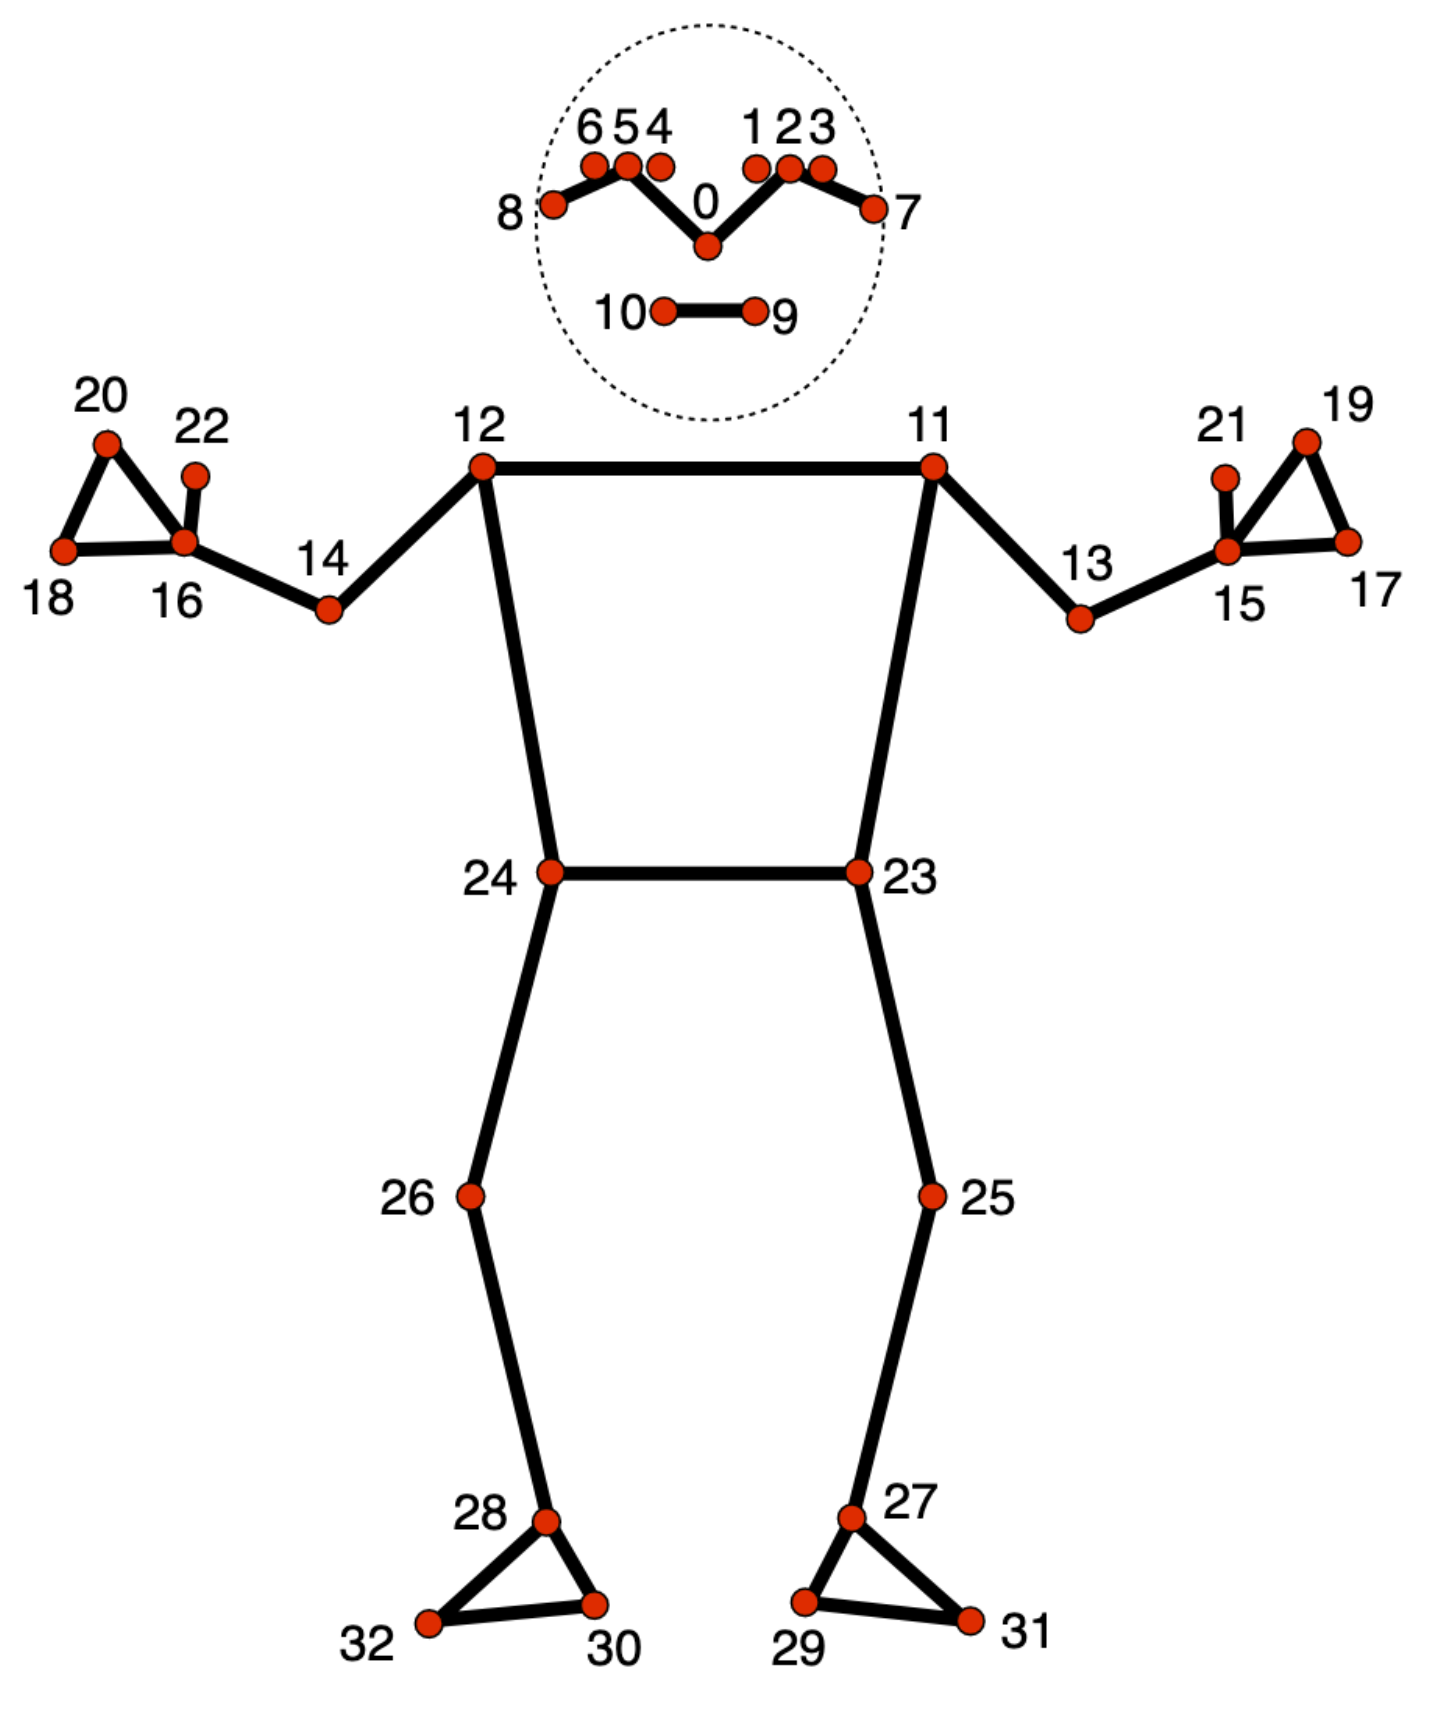
\includegraphics[width=0.6\textwidth, keepaspectratio]{imgs/mediapipe_landmarks.png}
\caption{A MediaPipe által detektált 33 térbeli landmark pontrendszere.}
\label{fig:mediapipe_landmarks}
\end{figure}

\section{Célkitűzések}
Jelen Tudományos Diákköri (TDK) munka célja egy olyan automatizált biomechanikai elemző szoftverrendszer kidolgozása, amely képes kosárlabda büntetődobások egyszerű videós felvételeiből kinematikai adatokat kinyerni marker nélküli pózbecslés segítségével. 
A kutatás során az alábbi célok kerültek megfogalmazásra:
\begin{itemize}
    \item A dobás szempontjából kritikus paraméterek (könyök-, váll- és térdszögek, elengedési pont) folyamatos nyomon követése a mozgás során.
    \item Egy gépi tanulási (Machine Learning) klasszifikációs modell betanítása, amely kísérletet tesz a dobás kimenetelének (sikeres vagy sikertelen) előrejelzésére a kinyert adatok alapján.
    \item Annak vizsgálata, hogy a modern számítógépes látásmódon alapuló technológiák (YOLO és MediaPipe) miként integrálhatók egy automatizált, edzőket és játékosokat támogató sportanalitikai rendszerbe.
\end{itemize}
